%%%%%%%%%%%%%%%%%%%%%%%%%%%%%%%%%%%%%%%%%
% Beamer Presentation
% LaTeX Template
% Version 1.0 (10/11/12)
%
% This template has been downloaded from:
% http://www.LaTeXTemplates.com
%
% License:
% CC BY-NC-SA 3.0 (http://creativecommons.org/licenses/by-nc-sa/3.0/)
%
%%%%%%%%%%%%%%%%%%%%%%%%%%%%%%%%%%%%%%%%%

%----------------------------------------------------------------------------------------
%	PACKAGES AND THEMES
%----------------------------------------------------------------------------------------

\documentclass{beamer}

\mode<presentation> {

% The Beamer class comes with a number of default slide themes
% which change the colors and layouts of slides. Below this is a list
% of all the themes, uncomment each in turn to see what they look like.

%\usetheme{default}
%\usetheme{AnnArbor}
%\usetheme{Antibes}
%\usetheme{Bergen}
%\usetheme{Berkeley}
%\usetheme{Berlin}
%\usetheme{Boadilla}
%\usetheme{CambridgeUS}
%\usetheme{Copenhagen}
%\usetheme{Darmstadt}
%\usetheme{Dresden}
%\usetheme{Frankfurt}
%\usetheme{Goettingen}
%\usetheme{Hannover}
%\usetheme{Ilmenau}
%\usetheme{JuanLesPins}
%\usetheme{Luebeck}
\usetheme{Madrid}
%\usetheme{Malmoe}
%\usetheme{Marburg}
%\usetheme{Montpellier}
%\usetheme{PaloAlto}
%\usetheme{Pittsburgh}
%\usetheme{Rochester}
%\usetheme{Singapore}
%\usetheme{Szeged}
%\usetheme{Warsaw}

% As well as themes, the Beamer class has a number of color themes
% for any slide theme. Uncomment each of these in turn to see how it
% changes the colors of your current slide theme.

%\usecolortheme{albatross}
%\usecolortheme{beaver}
%\usecolortheme{beetle}
%\usecolortheme{crane}
%\usecolortheme{dolphin}
%\usecolortheme{dove}
%\usecolortheme{fly}
%\usecolortheme{lily}
%\usecolortheme{orchid}
%\usecolortheme{rose}
%\usecolortheme{seagull}
%\usecolortheme{seahorse}
%\usecolortheme{whale}
%\usecolortheme{wolverine}

%\setbeamertemplate{footline} % To remove the footer line in all slides uncomment this line
%\setbeamertemplate{footline}[page number] % To replace the footer line in all slides with a simple slide count uncomment this line

%\setbeamertemplate{navigation symbols}{} % To remove the navigation symbols from the bottom of all slides uncomment this line
}

\usepackage{graphicx} % Allows including images
\usepackage{booktabs} % Allows the use of \toprule, \midrule and \bottomrule in tables
\usepackage[spanish]{babel}
\usepackage[utf8]{inputenc}
\usepackage{hyperref}
\usepackage{listings} % para agregar coloreado al codigo fuente
\lstset
{
    language=[LaTeX]TeX,
    breaklines=true,
    basicstyle=\tt\scriptsize,
    keywordstyle=\color{blue},
    identifierstyle=\color{magenta},
}

%----------------------------------------------------------------------------------------
%	TITLE PAGE
%----------------------------------------------------------------------------------------

\title[\LaTeX{}... ¿para que?]{Usando \LaTeX{} como herramienta para la creación de documentos académicos.} % The short title appears at the bottom of every slide, the full title is only on the title page

\author{Valentin Basel} % Your name
\institute[CIECS-UNC-CONICET] % Your institution as it will appear on the bottom of every slide, may be shorthand to save space
{
Universidad Nacional de Córdoba \\ % Your institution for the title page
\medskip
\textit{valentinbasel@gmail.com} % Your email address
}
\date{\today} % Date, can be changed to a custom date

\begin{document}

% presentación 1
\begin{frame}
  \titlepage % Print the title page as the first slide
    \begin{figure}
    \includegraphics[width=0.4\linewidth]{img/bysa.png}
  \end{figure}
\end{frame}

% presentación 2
\begin{frame}
\frametitle{\LaTeX{}}

  \begin{figure}
    
\includegraphics[width=0.8\linewidth]{img/fleco_y_male_latex.png}
  \end{figure}
\end{frame}

\begin{frame}
  \frametitle{Un poco de historia sobre \LaTeX{}}

\LaTeX{} es un sistema de composición de textos, orientado a la creación de documentos escritos que presenten una alta calidad tipográfica. Por sus características y posibilidades, es usado de forma especialmente intensa en la generación de artículos y libros científicos que incluyen, entre otros elementos, expresiones matemáticas.

\LaTeX{} está formado por un gran conjunto de macros de TeX, escrito por Leslie Lamport en 1984, con la intención de facilitar el uso del lenguaje de composición tipográfica, T E X, creado por Donald Knuth. Es muy utilizado para la composición de artículos académicos, tesis y libros técnicos, dado que la calidad tipográfica de los documentos realizados en LaTeX, se considera adecuada a las necesidades de una editorial científica de primera línea, muchas de las cuales ya lo emplean. 

\end{frame}

\begin{frame}
  \frametitle{Algunos detalles}
  \begin{itemize}
      \item \LaTeX{} Es un sistema para crear artículos académicos, tesis  libros científicos... y presentaciones como esta!
      \item \LaTeX{} \textbf{no es un programa}, es un lenguaje de composición de texto.
      \item Se usa un 'compilador' para generar los archivos PDFs desde archivos TEX.
      \item Hay muchos compiladores \LaTeX{}.
      \item Hay muchos Editores \LaTeX{}.
      \item Es muy diferente a trabajar con sistemas conocidos como WYSIWYG.
  \end{itemize}
\end{frame}


\begin{frame}
  \frametitle{WYSIWYG??????????????????????????????????????}
WYSIWYG, acrónimo de What You See Is What You Get (en español, "lo que ves es lo que obtienes"), es una frase aplicada a los procesadores de texto y otros editores de texto con formato (como los editores de HTML) que permiten escribir un documento mostrando directamente el resultado final, frecuentemente el resultado impreso.
\end{frame}

\begin{frame}
\frametitle{WYSIWYG}
Los procesadores de textos, como libreoffice o Microsoft Word son procesadores WYSIWYG. En contrapartida tenemos \LaTeX{} como un sistema \textbf{WYSIWYM}
  \begin{figure}
    \includegraphics[width=0.8\linewidth]{img/libreoffice.jpg}
  \end{figure}
\end{frame}

\begin{frame}
  \frametitle{WYSIWYM??????????????????????????????????????}
WYSIWYM es un acrónimo que significa “lo que ves es lo que quieres decir” (en inglés: What You See Is What You Mean). Es un paradigma para la creación de documentos alternativo al modelo (más difundido) WYSIWYG.

En este paradigma, el usuario se encarga de introducir los contenidos de forma estructurada siguiendo su valor semántico, en lugar de indicar su formato de representación final. 

La principal ventaja de este sistema es que se produce una total separación entre contenido y presentación. Por lo que el usuario sólo debe preocuparse de estructurar y agregar los contenidos, dejando los aspectos visuales a cargo del sistema de exportación. 
\end{frame}
\begin{frame}
\frametitle{\LaTeX{} es un sistema WYSIWYM}
nosotros escribimos código \LaTeX{}, en un archivo de texto plano (el clásico .txt) para luego compilar y generar nuestro archivo final (PDF por ejemplo).
  \begin{figure}
    \includegraphics[width=0.8\linewidth]{img/latex1.png}
  \end{figure}
\end{frame}


% frame de item
\begin{frame}
  \frametitle{Ventajas de LATEX}
  \begin{itemize}
      \item Composición de formulas matemáticas.
      \item Calidad de imprenta. Textos bien estructurados.Gráficos precisos y de calidad.
      \item instrucciones sencillas, estructura lógica; no necesita detalles visuales generalmente.
      \item Facilidad para estructuras complejas como bibliografía,indices, notas al pie, referencias cruzadas.
      \item Numerosos paquetes adicionales
      \item Independiente de la plataforma Linux, windows,.
      \item Gratuito y abierto.
      \item Salida postscript, PDF - imprentas, impresoras, web.
  \end{itemize}
\end{frame}

% frame de item
\begin{frame}
  \frametitle{Inconvenientes de LATEX}
  \begin{itemize}
    \item Curva de aprendizaje.
    \item Detectar errores.
    \item "Salir de la caja" puede ser una experiencia traumatizante.
  \end{itemize}
\end{frame}

\begin{frame}
\frametitle{entonces .... \LaTeX{}}

  \begin{figure}
    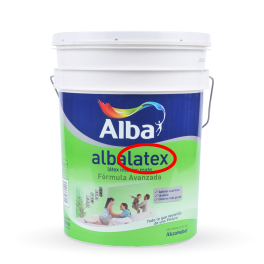
\includegraphics[width=0.8\linewidth]{img/alba_latex_final.png}
  \end{figure}
\end{frame}

\begin{frame}
  \frametitle{¿Que necesitamos para empezar?}
  Si bien pareciera un tema complejo, es relativamente simple instalar \LaTeX{} y que funcione
  en sistemas MS Windows (En los sistemas GNU/Linux es más fácil aun, por cierto).
  
  Lo que necesitamos es:
  
  \begin{itemize}
      \item Instalar los compiladores y paquetes de \LaTeX{}.
      \item Instalar un editor de código.
      \item Escribir nuestros archivos .tex
  \end{itemize}
\end{frame}



\begin{frame}
\frametitle{compiladores y paquetes de \LaTeX{} - MIKTEX}

  \textbf{https://miktex.org/download}
  \begin{figure}
    \includegraphics[width=0.8\linewidth]{img/miktex.png}
  \end{figure}
\end{frame}

\begin{frame}
\frametitle{Editores de código \LaTeX{} - TEXSTUDIO}

  \textbf{http://texstudio.sourceforge.net/}
  \begin{figure}
    \includegraphics[width=0.8\linewidth]{img/texstudio.png}
  \end{figure}
\end{frame}

\begin{frame}
\frametitle{Editores de código \LaTeX{} - TEXMAKER}
  \textbf{https://www.xm1math.net/texmaker/download.html}
  \begin{figure}
    \includegraphics[width=0.8\linewidth]{img/texmaker.png}
  \end{figure}
\end{frame}

\begin{frame}
\frametitle{Nuestro primer articulo en \LaTeX{} }
  \begin{figure}
    \includegraphics[width=0.8\linewidth]{img/latex1_texto.png}
  \end{figure}
\end{frame}

\begin{frame}
\frametitle{Preambulo}
En el preámbulo se escriben las instrucciones fundamentales que indican a L A T E X qué clase de documento se va a escribir y qué características va a tener éste, así como también las que indican a L A T E X qué paquetes se deben cargar. El preámbulo siempre empezará con la instrucción:
  \begin{figure}
    \includegraphics[width=0.8\linewidth]{img/instruccion.png}
  \end{figure}
\end{frame}
\begin{frame}
\frametitle{Paquetes}
Se llama paquete a una extensión del sistema básico que añade nuevas funciones. Hay, literalmente, cientos de paquetes con muy diversas funciones: inserción de imágenes (graphicx), paquetes gráficos (TikZ), internacionalización (babel, polyglossia), color (xcolor), música, ajedrez, ediciones críticas, secuencias de amninoácidos, etc. Todos estos paquetes deberán ser declarados con: 
  \begin{figure}
    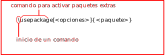
\includegraphics[width=0.8\linewidth]{img/instruccion2.png}
  \end{figure}
\end{frame}

\begin{frame}
\frametitle{Cuerpo}
El cuerpo del documento consiste en prácticamente todo lo que aparecerá en nuestra compilación. Es aquí, pues, donde escribiremos el texto verdadero.
  \begin{figure}
    \includegraphics[width=0.8\linewidth]{img/instruccion3.png}
  \end{figure}
\end{frame}

\begin{frame}
\frametitle{texto enriquecido}
Indudablemente podemos poner nuestro texto en \textbf{negrita}, \textit{cursiva}, \underline{subrayado}, y \textbf{\underline{\textit{todo junto al mismo tiempo}}}

  \begin{figure}
    
\includegraphics[width=0.8\linewidth]{img/instruccion4.png}
  \end{figure}
\end{frame}

\begin{frame}[fragile]
\frametitle{El documento mas simple que podemos hacer}
  \begin{lstlisting}
      \documentclass[12pt]{article}
      \begin{document}
      %aca es donde va nuestro texto
      \end{document}
  \end{lstlisting}
\end{frame}

\begin{frame}[fragile]
\frametitle{volviendo a ver documentclass}
Con la instrucción documentclass ordenamos como va a ser nuestro documento, definimos las opciones (tamaño de la fuente, orientación, tamaño del papel), y definimos su tipo (articulo, libro, reporte, presentación).
 
  \begin{lstlisting}
    \documentclass[option1, option2, etc.]{article}
  \end{lstlisting}
  
las opciones de documentclass:

  \begin{lstlisting}
    Font size (10pt, 11pt, 12pt)
    Paper size and format (a4paper, letterpaper, etc.)
    Draft mode (draft)
    Multiple columns (onecolumn, twocolumn)
    Formula-specific options (fleqn and leqno)
    Landscape print mode (landscape)
    Single- and double-sided documents (oneside, twoside)
    Titlepage behavior (notitlepage, titlepage)
    Chapter opening page (openright, openany)
  \end{lstlisting}

\end{frame}

\begin{frame}[fragile]
\frametitle{Hagamos un libro!}
  \begin{lstlisting}
      \documentclass[a4paper,11pt]{book}
      \usepackage[T1]{fontenc}
      \usepackage[utf8]{inputenc} % reconocer los acentos 
      \usepackage[spanish]{babel} % para traducciones. 
      \usepackage{lmodern}
      \title{}
      \author{}
      \begin{document}
      \maketitle
      \tableofcontents
      \chapter{}
        %aca empieza nuestro libro
      \end{document}
  \end{lstlisting}
\end{frame}

%% frame de imagenes
\begin{frame}
\frametitle{¿y las normas APA?}

  \begin{figure}
    \includegraphics[width=0.8\linewidth]{img/apa1.png}
  \end{figure}
\end{frame}

\begin{frame}[fragile]
  \frametitle{APA6}
Latex tiene muy buena integración con las normas APA. 

Para poder usarlas, tenemos que agregar los siguientes paquetes a nuestro preambulo:
  \begin{lstlisting}
      \usepackage{apacite} %normas APA
      \usepackage{natbib} % para poder citar correctamente
      \usepackage[hidelinks]{hyperref} % pdfs enriquecidos
      \bibliographystyle{apalike}% estilo APA
  \end{lstlisting}
\end{frame}
\begin{frame}
  \frametitle{como administrar las citas bibliográficas}
  
Latex reconoce las bases de datos BIBTEX, para poder administrar las citas bibliográficas.

Hacer una base de datos BITEX a mano puede ser una experiencia bastante fea, pero a no desesperar que 
tenemos una herramienta que ya lo resuelve todo.

\begin{center}
\textbf{ZOTERO}
\end{center}

Podemos gestionar nuestra base de datos de citas bibliográficas con zotero y luego exportar a formato bibtex para poder trabajar en latex

\end{frame}

\begin{frame}[fragile]
\frametitle{un ejemplo de bibtex}
  \begin{lstlisting}
  @book{association_for_computing_machinery_model_2004,
	address = {New York},
	title = {A {Model} {Curriculum} for {K}-12 {Computer} {Science}: {Final} {Report} of the {ACM} {K}-12 {Task} {Force} {Curriculum} {Committee}},
	isbn = {978-1-58113-837-5},
	shorttitle = {A {Model} {Curriculum} for {K}-12 {Computer} {Science}},
	language = {English},
	publisher = {ACM},
	author = {{Association for Computing Machinery}},
	year = {2004},
	note = {OCLC: 907036381}
  }
\end{lstlisting}

\end{frame}

\begin{frame}
\frametitle{¿y como se cita?}

  \begin{figure}
    \includegraphics[width=0.4\linewidth]{img/apa2.jpg}
  \end{figure}
\end{frame}

\begin{frame}[fragile]
\frametitle{vomo se cita en latex}
  \begin{lstlisting}
    \citet{john_iovine_robots_2002}
    \citep{eric_s._raymond_catedral_1998,karl_fogel_producir_2005}
    \citep{garrido__2009}
    \citep[pp 4]{sadosky2013cc}
\end{lstlisting}

\end{frame}

\begin{frame}
\frametitle{y el resultado seria}

John Iovine (2002)

(Eric S. Raymond, 1998; Karl Fogel, 2005)

(Garrido and Balaguer, 2009)

(Sadosky, 2013, pp 4)

\end{frame}

%% frame de imagenes
\begin{frame}
\frametitle{como quedan las referencias bibliográficas}

  \begin{figure}
    \includegraphics[width=0.8\linewidth]{img/referencias.png}
  \end{figure}
\end{frame}

% frame de imagenes
\begin{frame}[fragile]
\frametitle{FIN!!!!!!!!!!!!}

\begin{center}
\LARGE ¡GRACIAS!

\end{center}
\normalsize 

valentinbasel@gmail.com

\begin{lstlisting} 

https://github.com/valentinbasel/taller_latex 

\end{lstlisting}




\end{frame}

% frame de imagenes
%\begin{frame}
%\frametitle{}
%
%  \begin{figure}
%    \includegraphics[width=0.8\linewidth]{img/libreoffice.jpg}
%  \end{figure}
%\end{frame}

%% frame de texto
%\begin{frame}
%  \frametitle{}
%
%\end{frame}

%% frame de item
%\begin{frame}
%  \frametitle{}
%  \begin{itemize}
%      \item 
%  \end{itemize}
%\end{frame}
%----------------------------------------------------------------------------------------
\end{document} 
